\section[{Analytic functions in \irram}]{A datatype for analytic functions in \irram}
\subsection{Overview}
%\begin{frame}
%\frametitle{Classes}
%\code{POLY<coeff\_type>}
%\begin{itemize}
%\item<1-> A class for polynomials with coefficients of given type
%\item<2-> List of coefficients is internally represented as a vector
%\end{itemize}
% \onslide<3->{
%\code{POWERSERIES<coeff\_type>}
%}
%\begin{itemize}
%\item<3-> A class for powerseries
%\item<4-> Represented as a pointer to a sequence, i.e. a function from \code{INTEGER} to \code{coeff\_type}
%\end{itemize}
%\end{frame}
\begin{frame}[<+->]
\frametitle{Classes}
\code{BA\_ANA<coeff\_type>}
\begin{itemize}
\item A user-friendly class for analytic functions on a closed disc of rational radius
\item Standard operators \code{+}, \code{-}, \code{*} (both scalar multiplication and multiplication) are overloaded
\item Integration, Differentiation and Evaluation are implemented
\end{itemize}
\pause
\code{ANALYTIC\_RECT}
\begin{itemize}
\item A class for complex functions analytic on $[-1,1]$
\item Integration, Differentiation, Evaluation, \code{+},\code{-},  \code{*} also implemented  
\item Uses analytic continuation
\end{itemize}
\end{frame}
\subsection{Evaluation}
\begin{frame}
\frametitle{\code{BA\_ANA}: Evaluation}
			\begin{figure}[H]
				\centering
				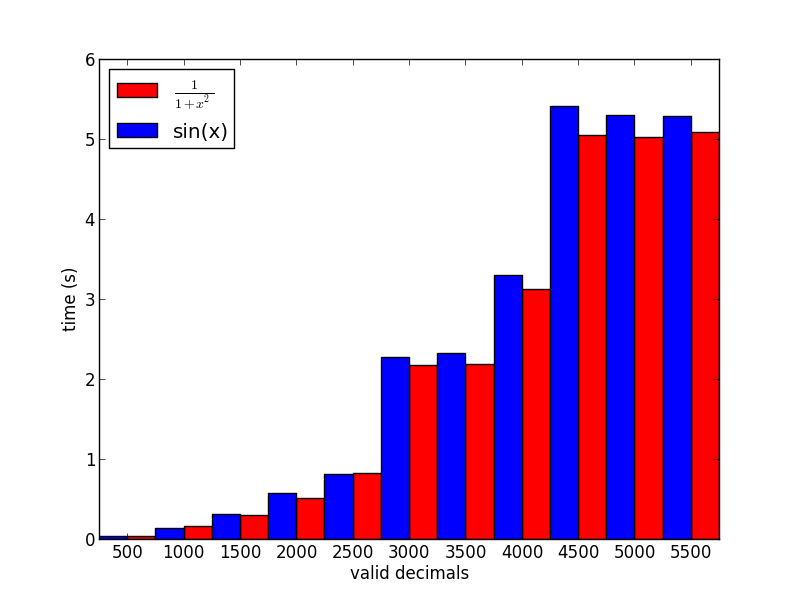
\includegraphics[width=0.7\textwidth]{ba_ana_dep_on_n_bar.png}
				\caption{running time evaluating \baana at fixed point $x=0.8$ depending on the desired number of valid decimals}
				\label{fig:ba_ana dep on n}
			\end{figure}
\end{frame}
\begin{frame}
\frametitle{\code{BA\_ANA}: Computing Derivatives}
			\begin{figure}[H]
				\centering
				\includegraphics[width=0.7\textwidth]{ba_ana_dep_on_diff_xinv.png}
        \caption{running time evaluating differentiated \baana with series for 
          $\frac{1}{1+x^2}$ at fixed point $x=0.8$ with different number
        of desired valid decimals depending on the number of differentiation}
				\label{fig:ba_ana dep on differentiation}
			\end{figure}
\end{frame}
\begin{frame}
\frametitle{\code{ANALYTIC\_RECT}: Dependency on $n$}
		\begin{figure}[h]
			\centering
			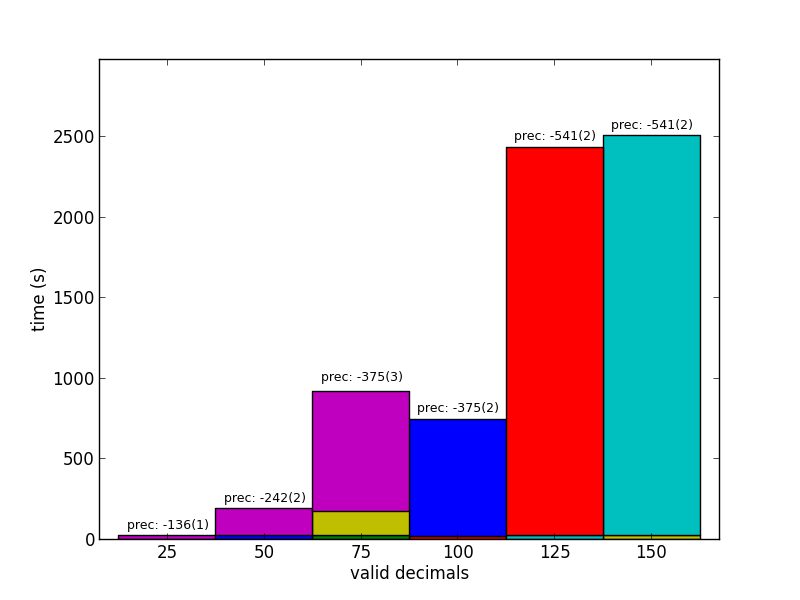
\includegraphics[width=0.7\textwidth]{sin_for_series_4_dep_on_n.png}
			\caption{running time of \anarect computing the sine function at the boundary of the third series, depending on the number of valid digits. }
			\label{fig:sin dep on n}
		\end{figure}
\end{frame}
\begin{frame}
  \frametitle{\code{ANALYTIC\_RECT}: Number of coefficients read}
		\begin{figure}[h]
			\centering
			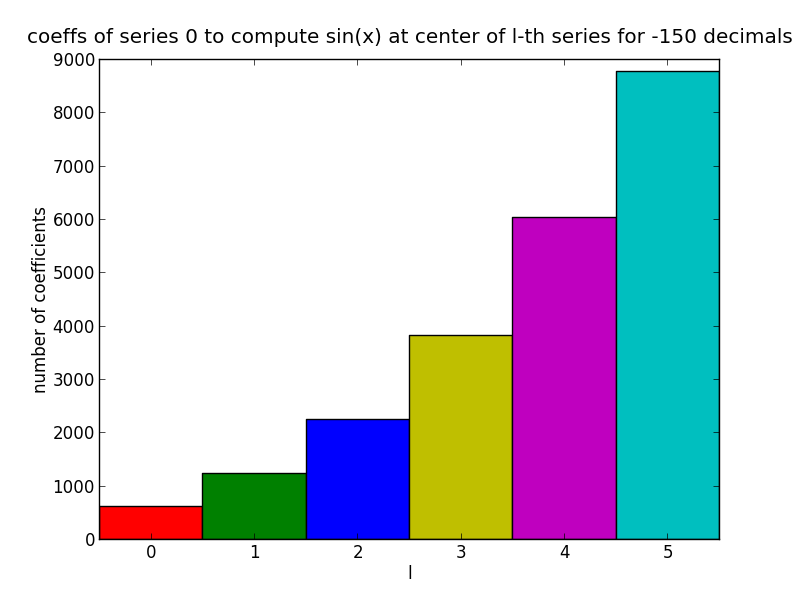
\includegraphics[width=0.7\textwidth]{sin_for_coeffs_prec_150_dep_on_series.png}
			\caption{Number of coefficients read from the original series when evaluating sine-function with 150 valid decimals, depending on the number of analytic continuations}
			\label{fig:sin dep on n}
		\end{figure}
\end{frame}
\begin{frame}
  \frametitle{\code{ANALYTIC\_RECT}: Dependency on continuations}
		\begin{figure}[h]
			\centering
				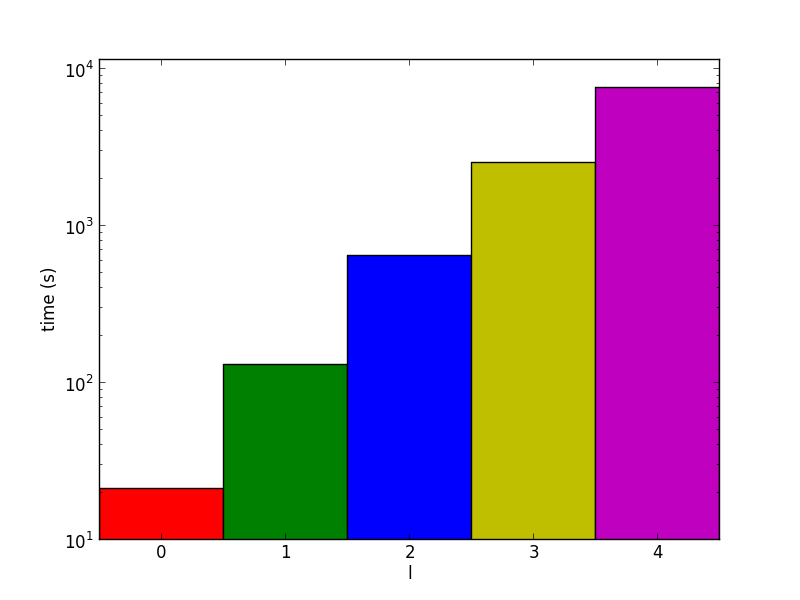
\includegraphics[width=0.7\textwidth]{sin_for_n_prec_150_dep_on_series_log.png}
			\caption{log-scale plot of the running time of evaluating the sine function for \anarect with 150 valid digits at the boundary of the $l$-th series.}
			\label{fig:baana dep on series}
		\end{figure}
\end{frame}
\section{Outlook}
\begin{frame}{ODEs}
	\vfill
	The following problem has been considered by multiple authors for polynomial right hand sides:
	\vfill
	Consider the ODE
	\[ h'(t) = f(t,h(t)), \quad h(0) = 0 \]\pause
	If $f$ is analytic, the solution $h$ will also be analytic.\pause
	\vfill
	The coeffiecient sequence of $h$ can be computed by a recursion.\pause
	\vfill
	If suitable constants for $f$ are specified, constants $A$ and $k$ for this sequence can be computed.\pause
	\vfill
	But: Our implementation does not support multivariate functions like $f$.\pause
\end{frame}


